\documentclass[12pt]{article}

\usepackage{fontspec}
\usepackage{xeCJK}
\usepackage{amsmath,amssymb}
\usepackage{geometry}
\usepackage{array}
\usepackage{booktabs}
\usepackage{tikz}
\usepackage{xcolor}

\IfFontExistsTF{Songti SC}
    {\setCJKmainfont{Songti SC}}
    {\setCJKmainfont{FandolSong-Regular}}
\IfFontExistsTF{Heiti SC}
    {\setCJKsansfont{Heiti SC}}
    {\setCJKsansfont{FandolHei-Regular}}
\IfFontExistsTF{Songti SC}
    {\setCJKmonofont{Songti SC}}
    {\setCJKmonofont{FandolSong-Regular}}

\geometry{a4paper,margin=1in}
\renewcommand{\arraystretch}{1.25}
\setlength{\parindent}{2em}

\begin{document}

\begin{center}
    {\LARGE\bfseries 编译原理作业 5\par}
    \vspace{1.0cm}
    {\large
    \begin{tabular}{rl}
    姓名：& 梁力航 \\
    学号：& 23336128 \\
    日期：& 2026年6月17日
    \end{tabular}\par}
\end{center}

\vspace{0.8cm}

%=============================================================================
\section*{第 1 题}

\subsection*{1.1 公共子表达式消除}

对基本块消除公共子表达式。左边为原指令，右边注明优化后调整的指令（未变指令不重写）。

\begin{center}
\begin{tabular}{lll}
\toprule
\multicolumn{2}{c}{\textbf{原指令}} & \textbf{优化后} \\
\midrule
(1) & $g = a + m$ & \\
(2) & $q = b * c$ & \\
(3) & $u = a + m$ & $u = g$ \quad（$a+m$ 已由(1)计算）\\
(4) & $d = a * a$ & \\
(5) & $a = 4 + b$ & \\
(6) & $h = b * c$ & $h = q$ \quad（$b*c$ 已由(2)计算）\\
\bottomrule
\end{tabular}
\end{center}

\textbf{说明}：子表达式 $a+m$ 在 (1) 和 (3) 中重复出现，$b*c$ 在 (2) 和 (6) 中重复出现。
消除公共子表达式后，(3) 直接复用 $g$，(6) 直接复用 $q$。注意 (5) 修改了 $a$ 的值，
但 $g = a+m$ 在 (5) 之前已经计算，所以 (3) 可以安全地使用 $g$。

\subsection*{1.2 复制传播、常量折叠与代数化简}

反复施用复制传播、常量折叠和代数化简。优化后的指令在右边注明。

\begin{center}
\begin{tabular}{lll}
\toprule
\multicolumn{2}{c}{\textbf{原指令}} & \textbf{优化后} \\
\midrule
(1) & $c = 4$ & \\
(2) & $t = a$ & \\
(3) & $m = b + t$ & $m = b + a$ \quad（复制传播：$t \to a$）\\
(4) & $p = c * c$ & $p = 16$ \quad（常量折叠：$4 \times 4 = 16$）\\
(5) & $i = x * 0$ & $i = 0$ \quad（代数化简：$x \times 0 = 0$）\\
(6) & $n = m * 2$ & \\
(7) & $e = c + p$ & $e = 20$ \quad（常量折叠：$4 + 16 = 20$）\\
(8) & $r = e + n$ & \\
\bottomrule
\end{tabular}
\end{center}

\textbf{优化过程说明}：
\begin{itemize}
    \item 第 (2)(3) 步——复制传播：$t = a$，因此将 $m = b + t$ 中的 $t$ 替换为 $a$，得到 $m = b + a$。
    \item 第 (4) 步——常量折叠：已知 $c = 4$（常量），故 $p = c * c = 4 \times 4 = 16$。
    \item 第 (5) 步——代数化简：利用代数恒等式 $x \times 0 = 0$，将 $i = x * 0$ 简化为 $i = 0$。
    \item 第 (7) 步——常量折叠：已知 $c = 4$、$p = 16$，故 $e = c + p = 4 + 16 = 20$。
    \item 第 (8) 步在优化后 $r = e + n = 20 + n$，其中 $n = m * 2$ 无法进一步简化（$m$ 非编译时常量）。
\end{itemize}

\subsection*{1.3 活跃变量分析}

基本块入口活跃变量集为 $\{x\}$，出口为 $\{s, e\}$，且基本块不包含死代码。
采用向后流分析（backward flow analysis），从出口向前逐条计算每个程序点的活跃变量集。

活跃变量计算规则：对于指令 $d = u\ op\ v$（或 $d = u$），
\[
\text{IN} = (\text{OUT} \setminus \{d\}) \cup \{u, v\}
\]
（若操作数为常量则可忽略，因其不在变量集合中。）

\begin{center}
\begin{tabular}{rclc}
\toprule
\multicolumn{3}{c}{\textbf{活 跃 变 量 分 析}} & \textbf{活跃变量集} \\
\midrule
    &         &                    & $\{x\}$ \\
(1) & $b = x * 0$  &                   & \\
    &         &                    & $\{b\}$ \\
(2) & $n = b$      &                   & \\
    &         &                    & $\{b, n\}$ \\
(3) & $a = b * 2$  &                   & \\
    &         &                    & $\{a, n\}$ \\
(4) & $e = a + n$  &                   & \\
    &         &                    & $\{e\}$ \\
(5) & $s = 2 + 3$  &                   & \\
    &         &                    & $\{s, e\}$ \\
\bottomrule
\end{tabular}
\end{center}

\textbf{计算步骤（从下往上）}：
\begin{enumerate}
    \item 出口处 $\{s, e\}$。第 (5) 条 $s = 2 + 3$ 定义 $s$，无变量使用，故 (5) 前为 $\{e\}$。
    \item 第 (4) 条 $e = a + n$ 定义 $e$，使用 $a,n$，故 (4) 前为 $\{a, n\}$。
    \item 第 (3) 条 $a = b * 2$ 定义 $a$，使用 $b$，故 (3) 前为 $\{b, n\}$。
    \item 第 (2) 条 $n = b$ 定义 $n$，使用 $b$，故 (2) 前为 $\{b\}$。
    \item 第 (1) 条 $b = x * 0$ 定义 $b$，使用 $x$，故 (1) 前为 $\{x\}$，与入口一致。$\checkmark$
\end{enumerate}

%=============================================================================
\section*{第 2 题}

\subsection*{2.1 基本块划分与流图}

\subsubsection*{基本块划分}

基本块的\textbf{首指令}（leader）规则：
(1) 第一条指令是首指令；
(2) 跳转目标指令是首指令；
(3) 紧跟在跳转指令之后的指令是首指令。

\begin{center}
\begin{tabular}{cll}
\toprule
\textbf{基本块} & \textbf{指令范围} & \textbf{内容简述} \\
\midrule
$B_1$ & 1--2  & $a = 0;\ b = 0$ \\
$B_2$ & 3     & $L_0\!: \mathbf{if}\ n/2\ \mathbf{goto}\ L_1$ \\
$B_3$ & 4--9  & $b = b + n;\ c = 4/2;\ t_1 = a*c;\ t_2 = c-1;\ a = a+t_2;\ \mathbf{goto}\ L_2$ \\
$B_4$ & 10--11 & $L_1\!: a = a + n;\ b = b + 1$ \\
$B_5$ & 12--13 & $L_2\!: n = n - 1;\ \mathbf{if}\ n > 0\ \mathbf{goto}\ L_0$ \\
$B_6$ & 14    & $\mathbf{return}\ a$ \\
\bottomrule
\end{tabular}
\end{center}

\subsubsection*{流图（Flow Graph）}

\begin{center}
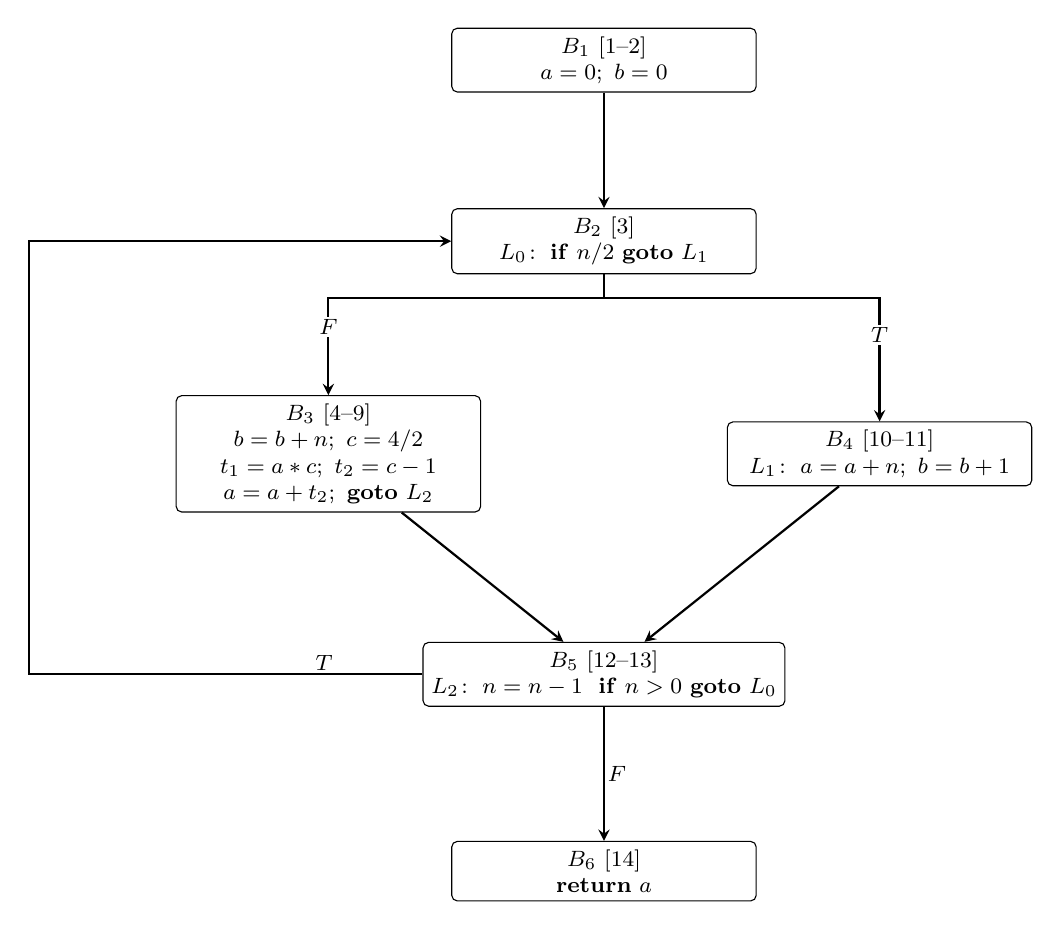
\begin{tikzpicture}[
    block/.style={
        rectangle, draw, rounded corners=2pt,
        minimum width=110pt, minimum height=12pt,
        align=center, font=\footnotesize, inner sep=3pt
    },
    arrow/.style={->, >=stealth, thick},
    lbl/.style={font=\footnotesize, inner sep=1pt, fill=white}
]

% Blocks — 增大垂直间距防止重叠
\node[block] (B1) at (0, 7.5)    {$B_1$ [1--2]\\$a=0;\ b=0$};
\node[block] (B2) at (0, 5.2)    {$B_2$ [3]\\$L_0\!:\ \mathbf{if}\ n/2\ \mathbf{goto}\ L_1$};
\node[block] (B3) at (-3.5, 2.5) {$B_3$ [4--9]\\$b=b+n;\ c=4/2$\\$t_1=a*c;\ t_2=c-1$\\$a=a+t_2;\ \mathbf{goto}\ L_2$};
\node[block] (B4) at (3.5, 2.5)  {$B_4$ [10--11]\\$L_1\!:\ a=a+n;\ b=b+1$};
\node[block] (B5) at (0, -0.3)   {$B_5$ [12--13]\\$L_2\!:\ n=n-1$\ \ $\mathbf{if}\ n>0\ \mathbf{goto}\ L_0$};
\node[block] (B6) at (0, -2.8)   {$B_6$ [14]\\$\mathbf{return}\ a$};

% Edges
\draw[arrow] (B1) -- (B2);
\draw[arrow] (B2.south) -- ++(0, -0.3) -| (B3.north) node[lbl, pos=0.65] {$F$};
\draw[arrow] (B2.south) -- ++(0, -0.3) -| (B4.north) node[lbl, pos=0.65] {$T$};
\draw[arrow] (B3) -- (B5);
\draw[arrow] (B4) -- (B5);
% 回边从左侧绕行，左移 5cm 确保垂直段在 B3 左侧之外
\draw[arrow] (B5.west) -- ++(-5, 0) node[lbl, pos=0.25, above] {$T$}
              |- (B2.west);
\draw[arrow] (B5) -- (B6) node[lbl, midway, right] {$F$};

\end{tikzpicture}
\end{center}

\textbf{说明}：
\begin{itemize}
    \item $B_2$ 中的指令 3 以 $n/2$ 为条件：当 $n/2 \neq 0$（即 $n \ge 2$ 或 $n \le -2$）时跳转到 $L_1$（$B_4$）；否则顺序进入 $B_3$。
    \item $B_3$ 以无条件跳转 $\mathbf{goto}\ L_2$ 结束，进入 $B_5$。
    \item $B_4$ 执行完后自然落入下方的 $L_2$（$B_5$）。
    \item $B_5$ 以 $n > 0$ 为条件：若真，回跳到 $L_0$（$B_2$）；若假，进入 $B_6$ 返回。
\end{itemize}

\subsection*{2.2 DAG 有向无环图}

将代码片段 4--8 转换为 DAG：

\[
\begin{array}{ll}
4: & b = b + n \\
5: & c = 4\ /\ 2 \\
6: & t_1 = a * c \\
7: & t_2 = c - 1 \\
8: & a = a + t_2
\end{array}
\]

DAG 构造过程中，常量表达式 $4/2 = 2$ 和 $2-1 = 1$ 可被常量折叠，
因此 $c$ 直接指向常量节点 $2$，$t_2$ 直接指向常量节点 $1$。

\begin{center}
\begin{tikzpicture}[
    circ/.style={circle, draw, inner sep=0pt, minimum size=14pt, font=\tiny},
    rect/.style={rectangle, draw, rounded corners=2pt, inner sep=2pt, font=\tiny},
    leaf/.style={font=\footnotesize},
    arrow/.style={->, >=stealth},
    level 1/.style={sibling distance=22mm},
    level 2/.style={sibling distance=14mm},
]

% DAG 整体居中
\node[circ] (plus1) at (0, 5)    {$+$};
\node[circ] (mult)  at (4.5, 5)  {$*$};
\node[circ] (plus2) at (9, 5)    {$+$};

\node[circ] (b0)    at (-1.2, 3) {$b_0$};
\node[circ] (n0)    at (1.2, 3)  {$n_0$};
\node[circ] (a0_1)  at (3.3, 3)  {$a_0$};
\node[circ] (c2)    at (5.7, 3)  {$2$};
\node[circ] (a0_2)  at (7.8, 3)  {$a_0$};
\node[circ] (t2_1)  at (10.2, 3) {$1$};

% Connect leaves to internal nodes
\draw[arrow] (plus1) -- (b0);
\draw[arrow] (plus1) -- (n0);
\draw[arrow] (mult) -- (a0_1);
\draw[arrow] (mult) -- (c2);
\draw[arrow] (plus2) -- (a0_2);
\draw[arrow] (plus2) -- (t2_1);

% Labels on internal nodes
\node[font=\footnotesize] at (0, 5.5)    {$b$};
\node[font=\footnotesize] at (4.5, 5.5)  {$t_1$};
\node[font=\footnotesize] at (9, 5.5)    {$a$};

% Labels on leaves
\node[font=\footnotesize] at (-1.2, 3.4) {$b_0$};
\node[font=\footnotesize] at (1.2, 3.4)  {$n_0$};
\node[font=\footnotesize] at (3.3, 3.4)  {$a_0$};
\node[font=\footnotesize] at (5.7, 3.4)  {$c$（常量2）};
\node[font=\footnotesize] at (7.8, 3.4)  {$a_0$};
\node[font=\footnotesize] at (10.2, 3.4) {$t_2$（常量1）};

\end{tikzpicture}
\end{center}

DAG 节点与指令的对应关系：

\begin{center}
\begin{tabular}{ccl}
\toprule
\textbf{指令} & \textbf{DAG 节点} & \textbf{说明} \\
\midrule
4: $b = b + n$   & $+$ 节点（子节点 $b_0$, $n_0$），结果标为 $b$ & 加法运算，无常量折叠 \\
5: $c = 4\ /\ 2$ & 常量 $2$，标为 $c$   & 常量折叠：$4/2 = 2$ \\
6: $t_1 = a * c$ & $*$ 节点（子节点 $a_0$, $2$），结果标为 $t_1$ & $c$ 已折叠为常量 $2$ \\
7: $t_2 = c - 1$ & 常量 $1$，标为 $t_2$ & 常量折叠：$2 - 1 = 1$ \\
8: $a = a + t_2$ & $+$ 节点（子节点 $a_0$, $1$），结果标为 $a$ & $t_2$ 已折叠为常量 $1$ \\
\bottomrule
\end{tabular}
\end{center}

\textbf{说明}：
\begin{itemize}
    \item 叶节点 $b_0$、$n_0$、$a_0$ 分别表示变量 $b$、$n$、$a$ 的初始值。
    \item 指令 5 的 $c = 4/2$ 在 DAG 构造时被常量折叠，$c$ 直接关联常量节点 $2$。
    \item 指令 7 的 $t_2 = c - 1 = 2 - 1$ 同样被常量折叠，$t_2$ 直接关联常量节点 $1$。
    \item 指令 6 的 $t_1 = a_0 * c = a_0 * 2$，使用常量节点 $2$。
    \item 指令 8 的 $a = a_0 + t_2 = a_0 + 1$，使用常量节点 $1$。
    \item $a_0$ 在 DAG 中出现两次（被 $t_1$ 和新的 $a$ 引用），体现了 DAG 的共享特性。
    \item 注意：最终 $a$ 的新值取决于 $t_2$ 而 $t_2=1$，因此 $a = a_0 + 1$，而非 $a = a_0 + t_2$。
\end{itemize}

\subsection*{2.3 代码优化方法}

对代码片段 4--8，可以应用以下两种优化方法：

\subsubsection*{方法一：常量折叠（Constant Folding）}

将编译时可计算出结果的常量表达式直接替换为其值。

\begin{center}
\begin{tabular}{lll}
\toprule
\textbf{原指令} & \textbf{优化后} & \textbf{说明} \\
\midrule
$c = 4\ /\ 2$   & $c = 2$   & $4/2$ 是编译时常量，直接计算为 $2$ \\
$t_2 = c - 1$   & $t_2 = 1$ & $c$ 已折叠为 $2$，$2-1=1$ 也是编译时常量 \\
\bottomrule
\end{tabular}
\end{center}

\subsubsection*{方法二：常量传播（Constant Propagation）}

将已知的常量值传播到使用该变量的指令中，以发现更多优化机会。

\begin{center}
\begin{tabular}{lll}
\toprule
\textbf{原指令} & \textbf{优化后} & \textbf{说明} \\
\midrule
$t_1 = a * c$   & $t_1 = a * 2$ & $c$ 已折叠为常量 $2$，传播到此处 \\
$a = a + t_2$   & $a = a + 1$   & $t_2$ 已折叠为常量 $1$，传播到此处 \\
\bottomrule
\end{tabular}
\end{center}

\textbf{优化效果}：经过常量折叠和常量传播后，原 5 条指令中的 4 条得到了简化，
消除了两次除法、一次减法和两次不必要变量引用，指令执行效率明显提高。

\end{document}
